\chapter{Casistica, materiali e metodi}

\section{Casistica}

\section{Materiali e metodi}

\subsection{Valutazione auxologica}

\begin{figure}[h]
  \begin{center}
      \includegraphics{grafici/centili/centili.eps} %\\
  \end{center}
  \caption{Standard antropometrici neonatali relativi a peso ed altezza nell'Italia nord-orientale}
\end{figure}

\begin{figure}[h]
  \begin{center}
	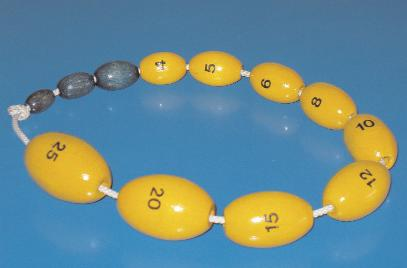
\includegraphics{grafici/orchidometro.jpg}
  \end{center}
  \caption{Orchidometro di Prader}
\end{figure}

\begin{figure}[h]
  \begin{center}
	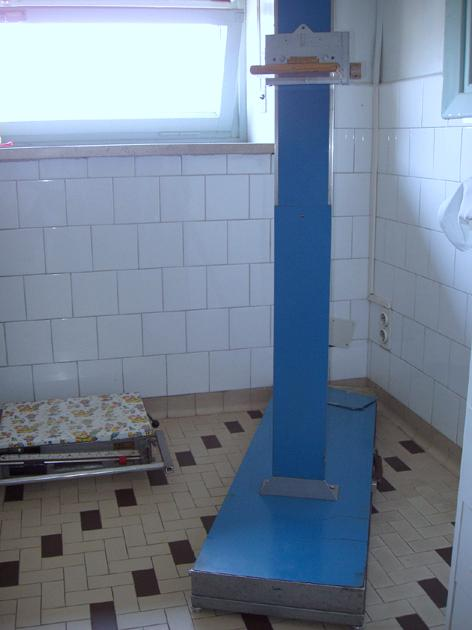
\includegraphics{grafici/statimetro.jpg}
  \end{center}
  \caption{Statimetro di Harpenden}
\end{figure}

\subsection{Valutazione ormonale}

\subsection{Analisi statistiche}
